\documentclass{article}
\usepackage{quiver}
\usepackage{tikz}
\usepackage{tikz-cd}
\usepackage{amsmath}
\usetikzlibrary{positioning, shapes.geometric, arrows.meta}

\begin{document}

\begin{equation*}
\begin{tikzcd}[ampersand replacement=\&,sep=normal, cells={nodes={draw, minimum width=1cm, minimum height=0.5cm, anchor=center}}]
	\&\&\&\&\&\&\& Self \\
	\\
	\&\&\&\&\&\&\& Intellect \\
	\\
	\&\&\&\&\&\&\& {Slow Mind} \\
	\\
	\&\&\&\&\&\&\& Ego \\
	Nature \&\& Object \&\& Body \&\&\&\&\&\& Soul \&\& Subject \&\& Culture \\
	\&\&\&\&\&\&\& Socio \\
	\\
	\&\&\&\&\&\&\& {Fast Mind} \\
	\\
	\&\&\&\&\&\&\& Life \\
	\\
	\&\&\&\&\&\&\& Death
	\arrow["Motivatio", from=1-8, to=8-13]
	\arrow["Decisio"{description}, from=3-8, to=1-8]
	\arrow["Cognitio"{description}, from=5-8, to=3-8]
	\arrow["Emotio", from=5-8, to=8-11]
	\arrow["Emotio"{description}, from=7-8, to=8-11]
	\arrow["Vinculum"{description}, tail reversed, from=7-8, to=9-8]
	\arrow["Emergentio", from=8-1, to=8-3]
	\arrow["Observatio", squiggly, from=8-3, to=1-8]
	\arrow["Sensatio", from=8-3, to=8-5]
	\arrow["Preservatio"', squiggly, from=8-3, to=15-8]
	\arrow["Interpratatio", from=8-5, to=5-8]
	\arrow["Conditio"{description}, from=8-5, to=7-8]
	\arrow["Intuitio"', from=8-5, to=11-8]
	\arrow["Motivatio", from=8-11, to=8-13]
	\arrow["Expressio"{description}, from=8-11, to=9-8]
	\arrow["Creatio", from=8-13, to=8-15]
	\arrow["{Sensatio`}"{description}, from=9-8, to=8-5]
	\arrow["Emotio"', from=11-8, to=8-11]
	\arrow["Memorizatio"{description}, from=11-8, to=13-8]
	\arrow["Instictio"{description}, from=13-8, to=15-8]
	\arrow["Motivatio"', from=15-8, to=8-13]
\end{tikzcd}
\end{equation*}

\begin{center}
\begin{equation*}
\resizebox{1.4\textwidth}{!}{
\begin{tikzcd}[ampersand replacement=\&,sep=normal, cells={nodes={draw, minimum width=1cm, minimum height=0.5cm, anchor=center}}]
    \&\&\&\&\&\&\& Self \\
    \\
    \&\&\&\&\&\&\& Intellect \\
    \\
    \&\&\&\&\&\&\& {Slow Mind} \\
    \\
    \&\&\&\&\&\&\& Ego \\
    Nature \&\& Object \&\& Body \&\&\&\&\&\& Soul \&\& Subject \&\& Culture \\
    \&\&\&\&\&\&\& Socio \\
    \\
    \&\&\&\&\&\&\& {Fast Mind} \\
    \\
    \&\&\&\&\&\&\& Life \\
    \\
    \&\&\&\&\&\&\& Death
    \arrow["Motivatio", from=1-8, to=8-13]
    \arrow["Decisio"{description}, from=3-8, to=1-8]
    \arrow["Cognitio"{description}, from=5-8, to=3-8]
    \arrow["Emotio", from=5-8, to=8-11]
    \arrow["Emotio"{description}, from=7-8, to=8-11]
    \arrow["Vinculum"{description}, tail reversed, from=7-8, to=9-8]
    \arrow["Emergentio", from=8-1, to=8-3]
    \arrow["Observatio", squiggly, from=8-3, to=1-8]
    \arrow["Sensatio", from=8-3, to=8-5]
    \arrow["Preservatio"', squiggly, from=8-3, to=15-8]
    \arrow["Interpratatio", from=8-5, to=5-8]
    \arrow["Conditio"{description}, from=8-5, to=7-8]
    \arrow["Intuitio"', from=8-5, to=11-8]
    \arrow["Motivatio", from=8-11, to=8-13]
    \arrow["Expressio"{description}, from=8-11, to=9-8]
    \arrow["Creatio", from=8-13, to=8-15]
    \arrow["{Sensatio`}"{description}, from=9-8, to=8-5]
    \arrow["Emotio"', from=11-8, to=8-11]
    \arrow["Memorizatio"{description}, from=11-8, to=13-8]
    \arrow["Instictio"{description}, from=13-8, to=15-8]
    \arrow["Motivatio"', from=15-8, to=8-13]
\end{tikzcd}
}
\end{equation*}
\end{center}


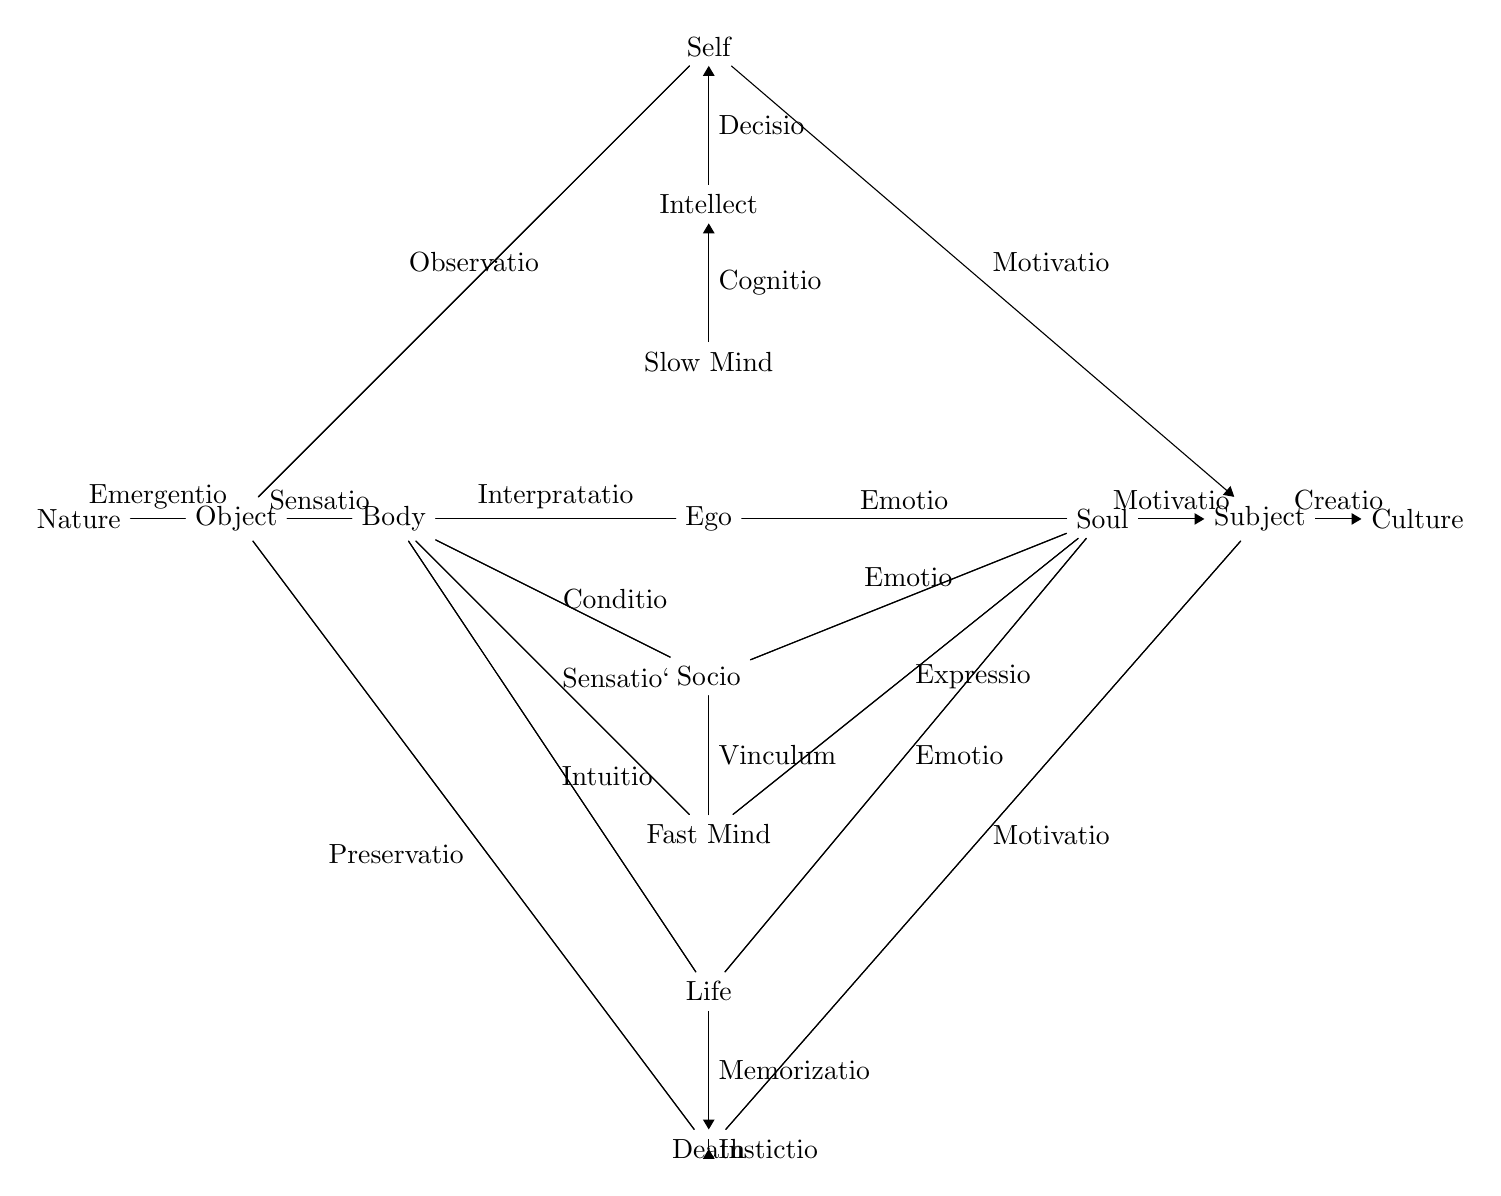
\begin{tikzpicture}[ampersand replacement=\&]
    % Define nodes
	\node (Self) at (8, 10) {Self};
	\node (Intellect) at (8, 8) {Intellect};
	\node (SlowMind) at (8, 6) {Slow Mind};
	\node (Ego) at (8, 4) {Ego};
	\node (Soul) at (13, 4) {Soul};
	\node (Socio) at (8, 2) {Socio};
	\node (FastMind) at (8, 0) {Fast Mind};
	\node (Life) at (8, -2) {Life};
	\node (Death) at (8, -4) {Death};
	\node (Nature) at (0, 4) {Nature};
	\node (Object) at (2, 4) {Object};
	\node (Body) at (4, 4) {Body};
	\node (Subject) at (15, 4) {Subject};
	\node (Culture) at (17, 4) {Culture};

    % Define crow's foot notation
    \tikzset{
        crowsfoot one/.style={
            to path={-- ++(0.2,-0.2) -- ++(-0.2,0.2) -- ++(0.2,0.2) \tikztonodes},
            postaction={draw, line cap=round}
        },
        crowsfoot many/.style={
            to path={-- ++(0.2,-0.2) -- ++(-0.2,0.2) -- ++(0.2,0.2) -- ++(-0.2,-0.2) \tikztonodes},
            postaction={draw, line cap=round}
        }
    }

    % Draw relationships using custom crow's foot notation
	\draw[-{Triangle[scale=1.0]}] (Self) -- node[above right] {Motivatio} (Subject);
	\draw[-{Triangle[scale=1.0]}] (Intellect) -- node[right] {Decisio} (Self);
	\draw[-{Triangle[scale=1.0]}] (SlowMind) -- node[right] {Cognitio} (Intellect);
	\draw[crowsfoot one] (Ego) -- node[above] {Emotio} (Soul);
	\draw[crowsfoot one] (Socio) -- node[above] {Emotio} (Soul);
	\draw[crowsfoot one] (Socio) -- node[right] {Vinculum} (FastMind);
	\draw[crowsfoot many] (Nature) -- node[above] {Emergentio} (Object);
	\draw[crowsfoot many] (Object) -- node[above] {Observatio} (Self);
	\draw[crowsfoot many] (Object) -- node[above] {Sensatio} (Body);
	\draw[crowsfoot many] (Object) -- node[below left] {Preservatio} (Death);
	\draw[crowsfoot one] (Body) -- node[above] {Interpratatio} (Ego);
	\draw[crowsfoot one] (Body) -- node[right] {Conditio} (Socio);
	\draw[crowsfoot one] (Body) -- node[below right] {Intuitio} (Life);
	\draw[-{Triangle[scale=1.0]}] (Soul) -- node[above] {Motivatio} (Subject);
	\draw[crowsfoot one] (Soul) -- node[right] {Expressio} (FastMind);
	\draw[-{Triangle[scale=1.0]}] (Subject) -- node[above] {Creatio} (Culture);
	\draw[crowsfoot one] (FastMind) -- node[right] {Sensatio`} (Body);
	\draw[crowsfoot one] (Life) -- node[right] {Emotio} (Soul);
	\draw[-{Triangle[scale=1.0]}] (Life) -- node[right] {Memorizatio} (Death);
	\draw[-{Triangle[scale=1.0]}] (Death) -- node[right] {Instictio} (Death);
	\draw[crowsfoot one] (Death) -- node[right] {Motivatio} (Subject);
\end{tikzpicture}

\end{document}


\end{document}
